	%-=-=-=-=-=-=-=-=-=-=-=-=-=-=-=-=-=-=-=-=-=-=-=-=
%
%        LOADING DOCUMENT
%
%-=-=-=-=-=-=-=-=-=-=-=-=-=-=-=-=-=-=-=-=-=-=-=-=

\documentclass[newPxFont,pagenumber]{beamer}
\usetheme{sthlm}
%\usecolortheme{sthlmv42}

%-=-=-=-=-=-=-=-=-=-=-=-=-=-=-=-=-=-=-=-=-=-=-=-=
%        LOADING PACKAGES
%-=-=-=-=-=-=-=-=-=-=-=-=-=-=-=-=-=-=-=-=-=-=-=-=
\usepackage[utf8]{inputenc}
\usepackage[frenchb]{babel}
\usepackage[normalem]{ulem}
\makeatletter
\newcommand*{\currentname}{\@currentlabelname}
\makeatother

\graphicspath{ {fig/} }
% add page number

\setbeamerfont{title}{series=\upshape}
\setbeamertemplate{footline}{\hfill\footnotesize\insertframenumber\hskip3pt\null\vskip3pt}

\newcommand{\argmax}{\mathop{\mathrm{argmax}}\limits}
\renewcommand{\max}{\mathop{\mathrm{max}}\limits}

\addto\captionsfrench{%
\renewcommand{\figurename}{\scriptsize {\scshape Figure}}
\renewcommand{\tablename}{\scriptsize {\scshape Table}}
}

%-=-=-=-=-=-=-=-=-=-=-=-=-=-=-=-=-=-=-=-=-=-=-=-=
%        BEAMER OPTIONS
%-=-=-=-=-=-=-=-=-=-=-=-=-=-=-=-=-=-=-=-=-=-=-=-=

%\setbeameroption{show notes}
\setbeamersize{text margin left=1pt,text margin right=1pt}

%-=-=-=-=-=-=-=-=-=-=-=-=-=-=-=-=-=-=-=-=-=-=-=-=
%
%	PRESENTATION INFORMATION
%
%-=-=-=-=-=-=-=-=-=-=-=-=-=-=-=-=-=-=-=-=-=-=-=-=

\title{\normalsize AgroLD: une plateforme de données liées pour
	comprendre les interactions génotype-phénotype
	des plantes}
\subtitle{\scriptsize AGAPIADES 2019 -- \textit{20 mai 2019}}
%\date{\small{\jobname}}
\date{\scriptsize Début de mission: 07 janvier 2019}
\author{\normalsize Gildas Tagny Ngompé (INRA - UMR AGAP - Equipe ID)}
\institute{\scriptsize \textbf{Direction de thèse:} \begin{itemize}
\item Pierre Larmande (IRD - UMR DIADE)
\item Manuel Ruiz (CIRAD - UMR AGAP - Equipe ID)
\end{itemize}
}

\hypersetup{
pdfauthor = {\author{}: tagnyngompe@gmail.com},
pdfsubject = {},
pdfkeywords = {},
pdfmoddate= {D:\pdfdate},
pdfcreator = {}
}

\begin{document}
\nocite{}
%-=-=-=-=-=-=-=-=-=-=-=-=-=-=-=-=-=-=-=-=-=-=-=-=
%
%	TITLE PAGE
%
%-=-=-=-=-=-=-=-=-=-=-=-=-=-=-=-=-=-=-=-=-=-=-=-=
\begin{frame}[plain]
	\titlepage
\end{frame}
%}
%-=-=-=-=-=-=-=-=-=-=-=-=-=-=-=-=-=-=-=-=-=-=-=-=
%
%	TABLE OF CONTENTS: Plan
%
%-=-=-=-=-=-=-=-=-=-=-=-=-=-=-=-=-=-=-=-=-=-=-=-=
\section*{Plan}
\begin{frame}[c]{\currentname}
\tableofcontents[hideallsubsections]
\end{frame}

%-=-=-=-=-=-=-=-=-=-=-=-=-=-=-=-=-=-=-=-=-=-=-=-=
%	Introduction: 
%-=-=-=-=-=-=-=-=-=-=-=-=-=-=-=-=-=-=-=-=-=-=-=-=

\section{AgroLD}


\begin{frame}{Quoi?}
\begin{columns}
\begin{column}{0.25\textwidth}
	\small
\begin{itemize}
\item Intégration de données biologiques agronomiques
\item Uniformisation en RDF
\item Publication web
\end{itemize}	

\end{column}
\begin{column}{0.75\textwidth}
\centering \includegraphics[scale=0.3]{ResourcesDiagram.png}
\end{column}
\end{columns}
\end{frame}

\begin{frame}{Comment?}

\centering 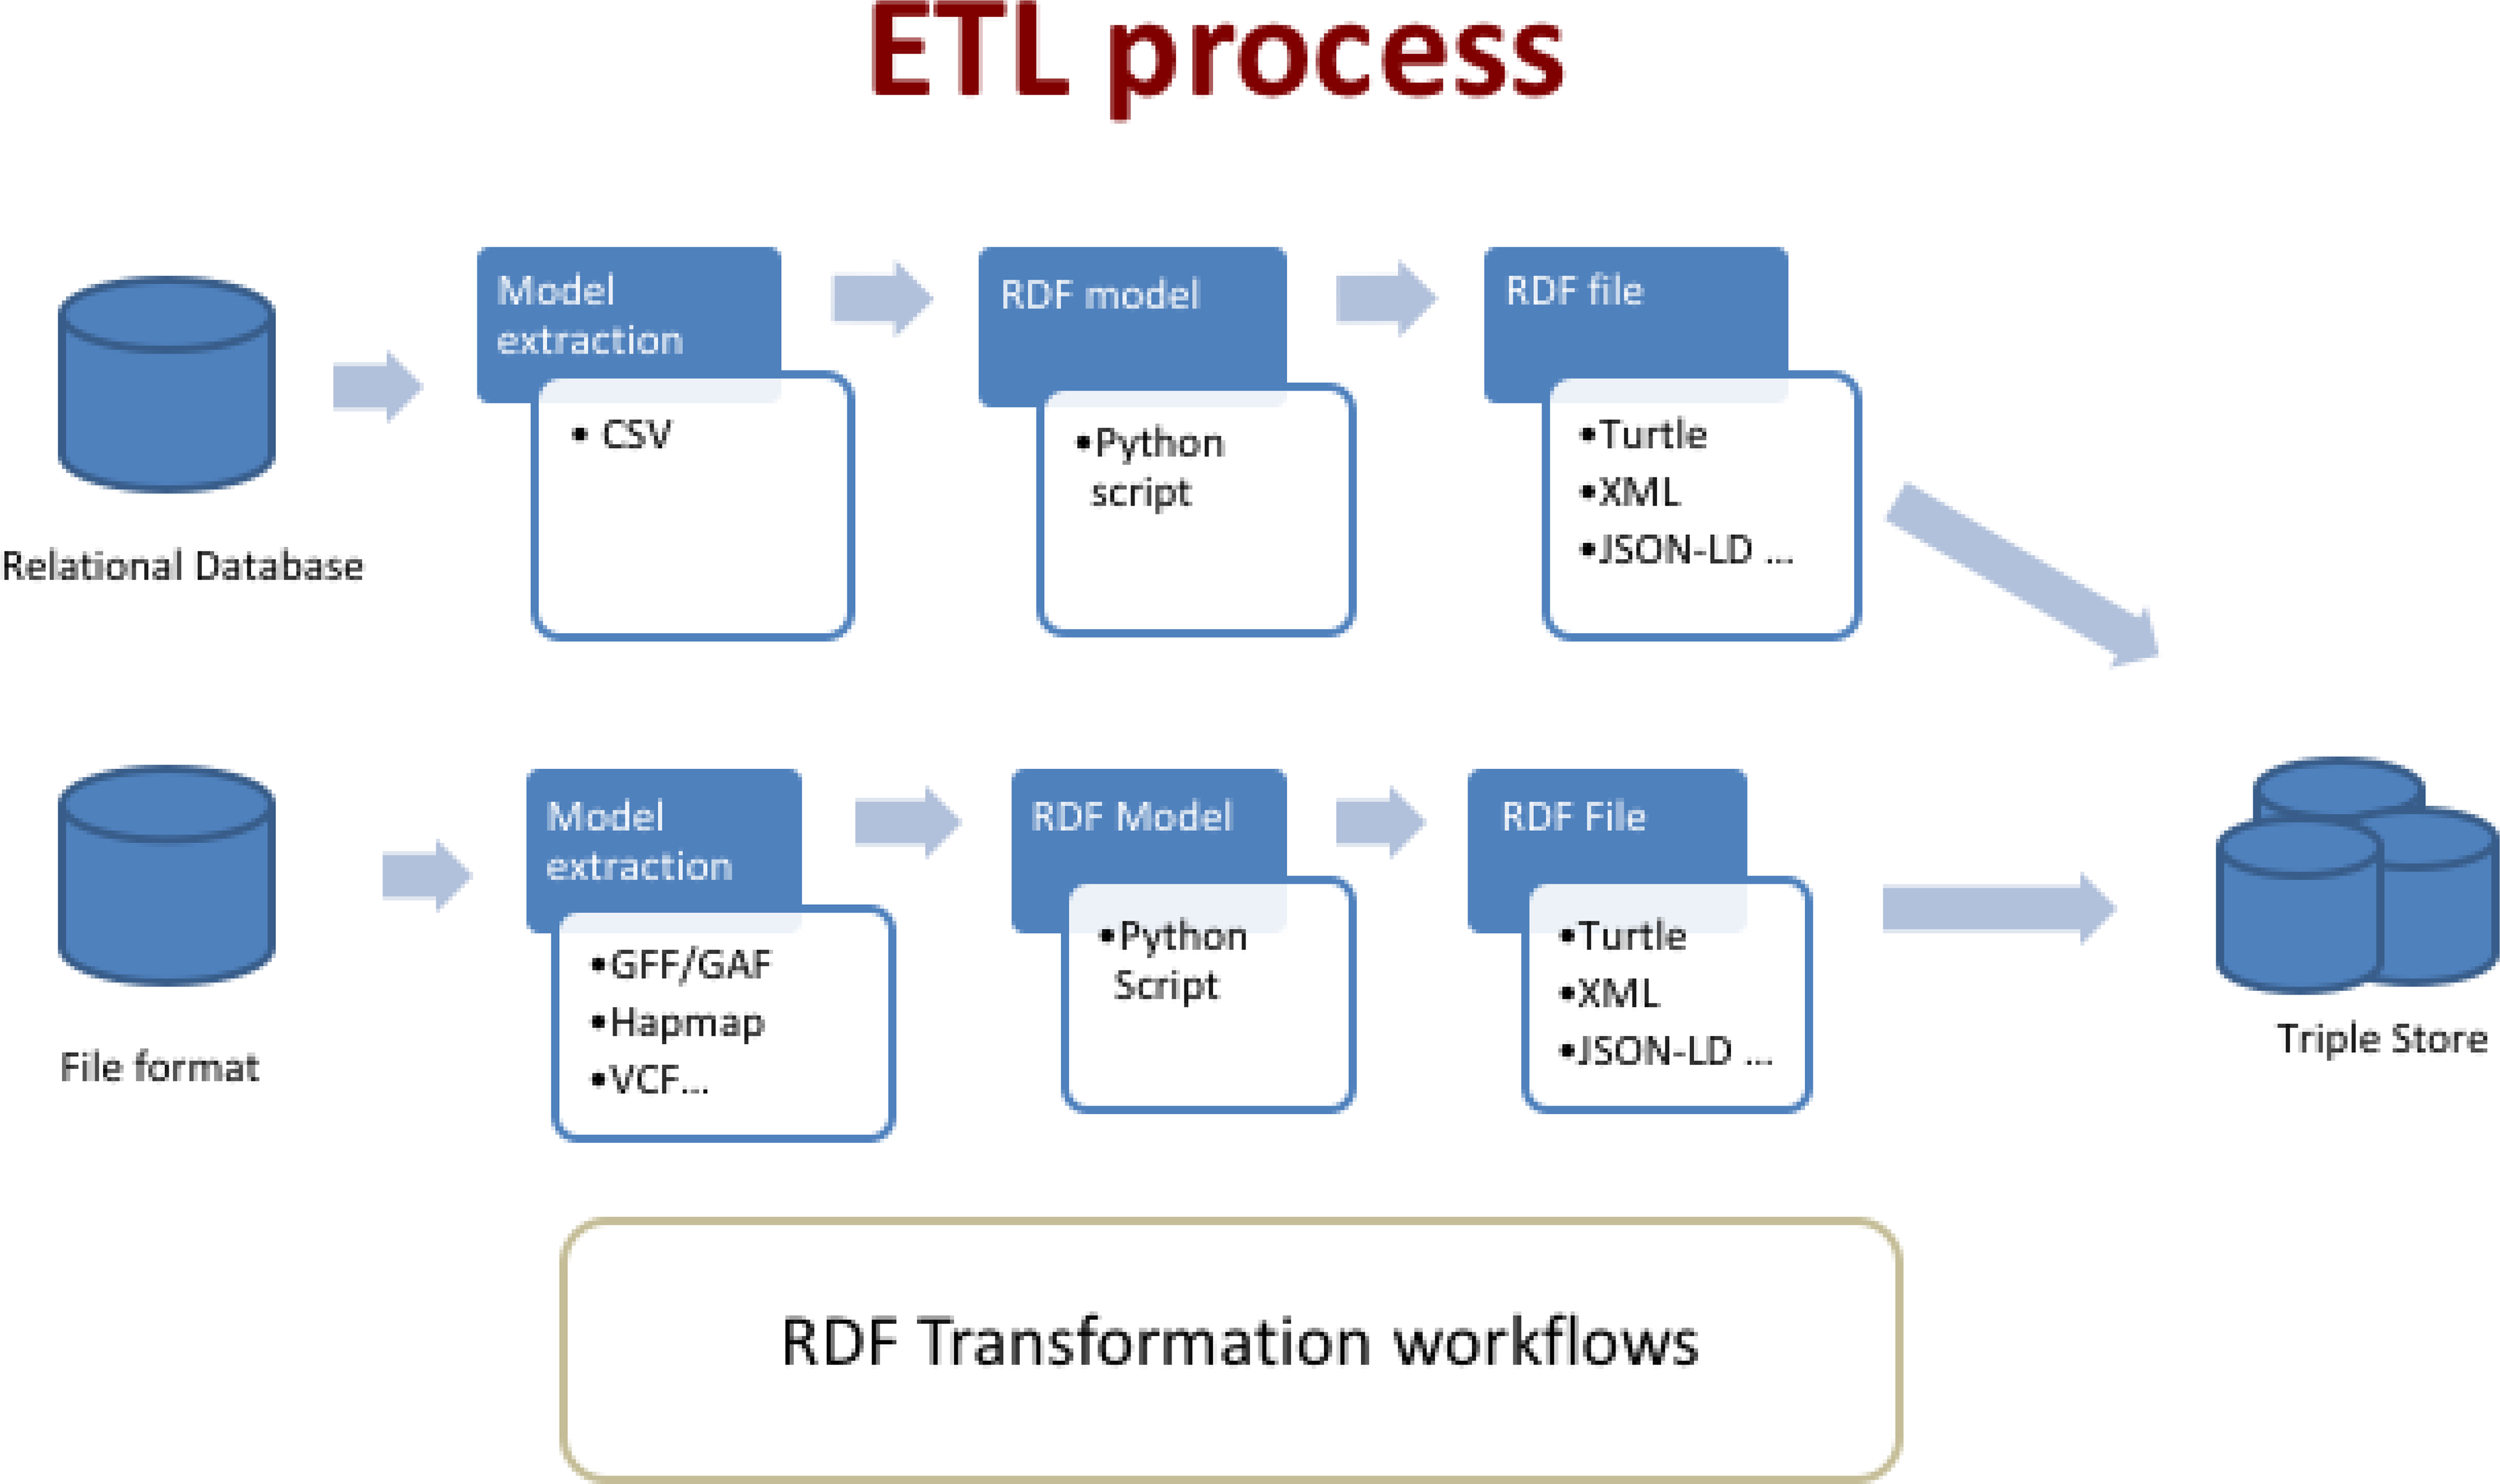
\includegraphics[width=0.7\textwidth]{data2rdf-agrold.png}
\end{frame}

\begin{frame}{Comment?}

\centering 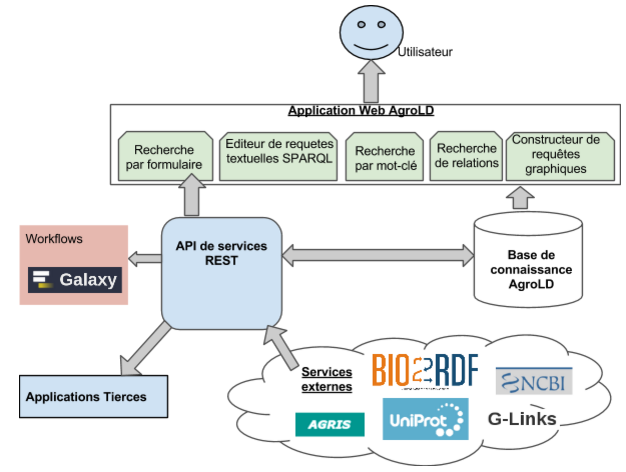
\includegraphics[width=0.8\textwidth]{archAgrold.png}
\end{frame}

\begin{frame}{Où?}

\url{http://agrold.southgreen.fr} ou \url{http://agrold.org}

\centering 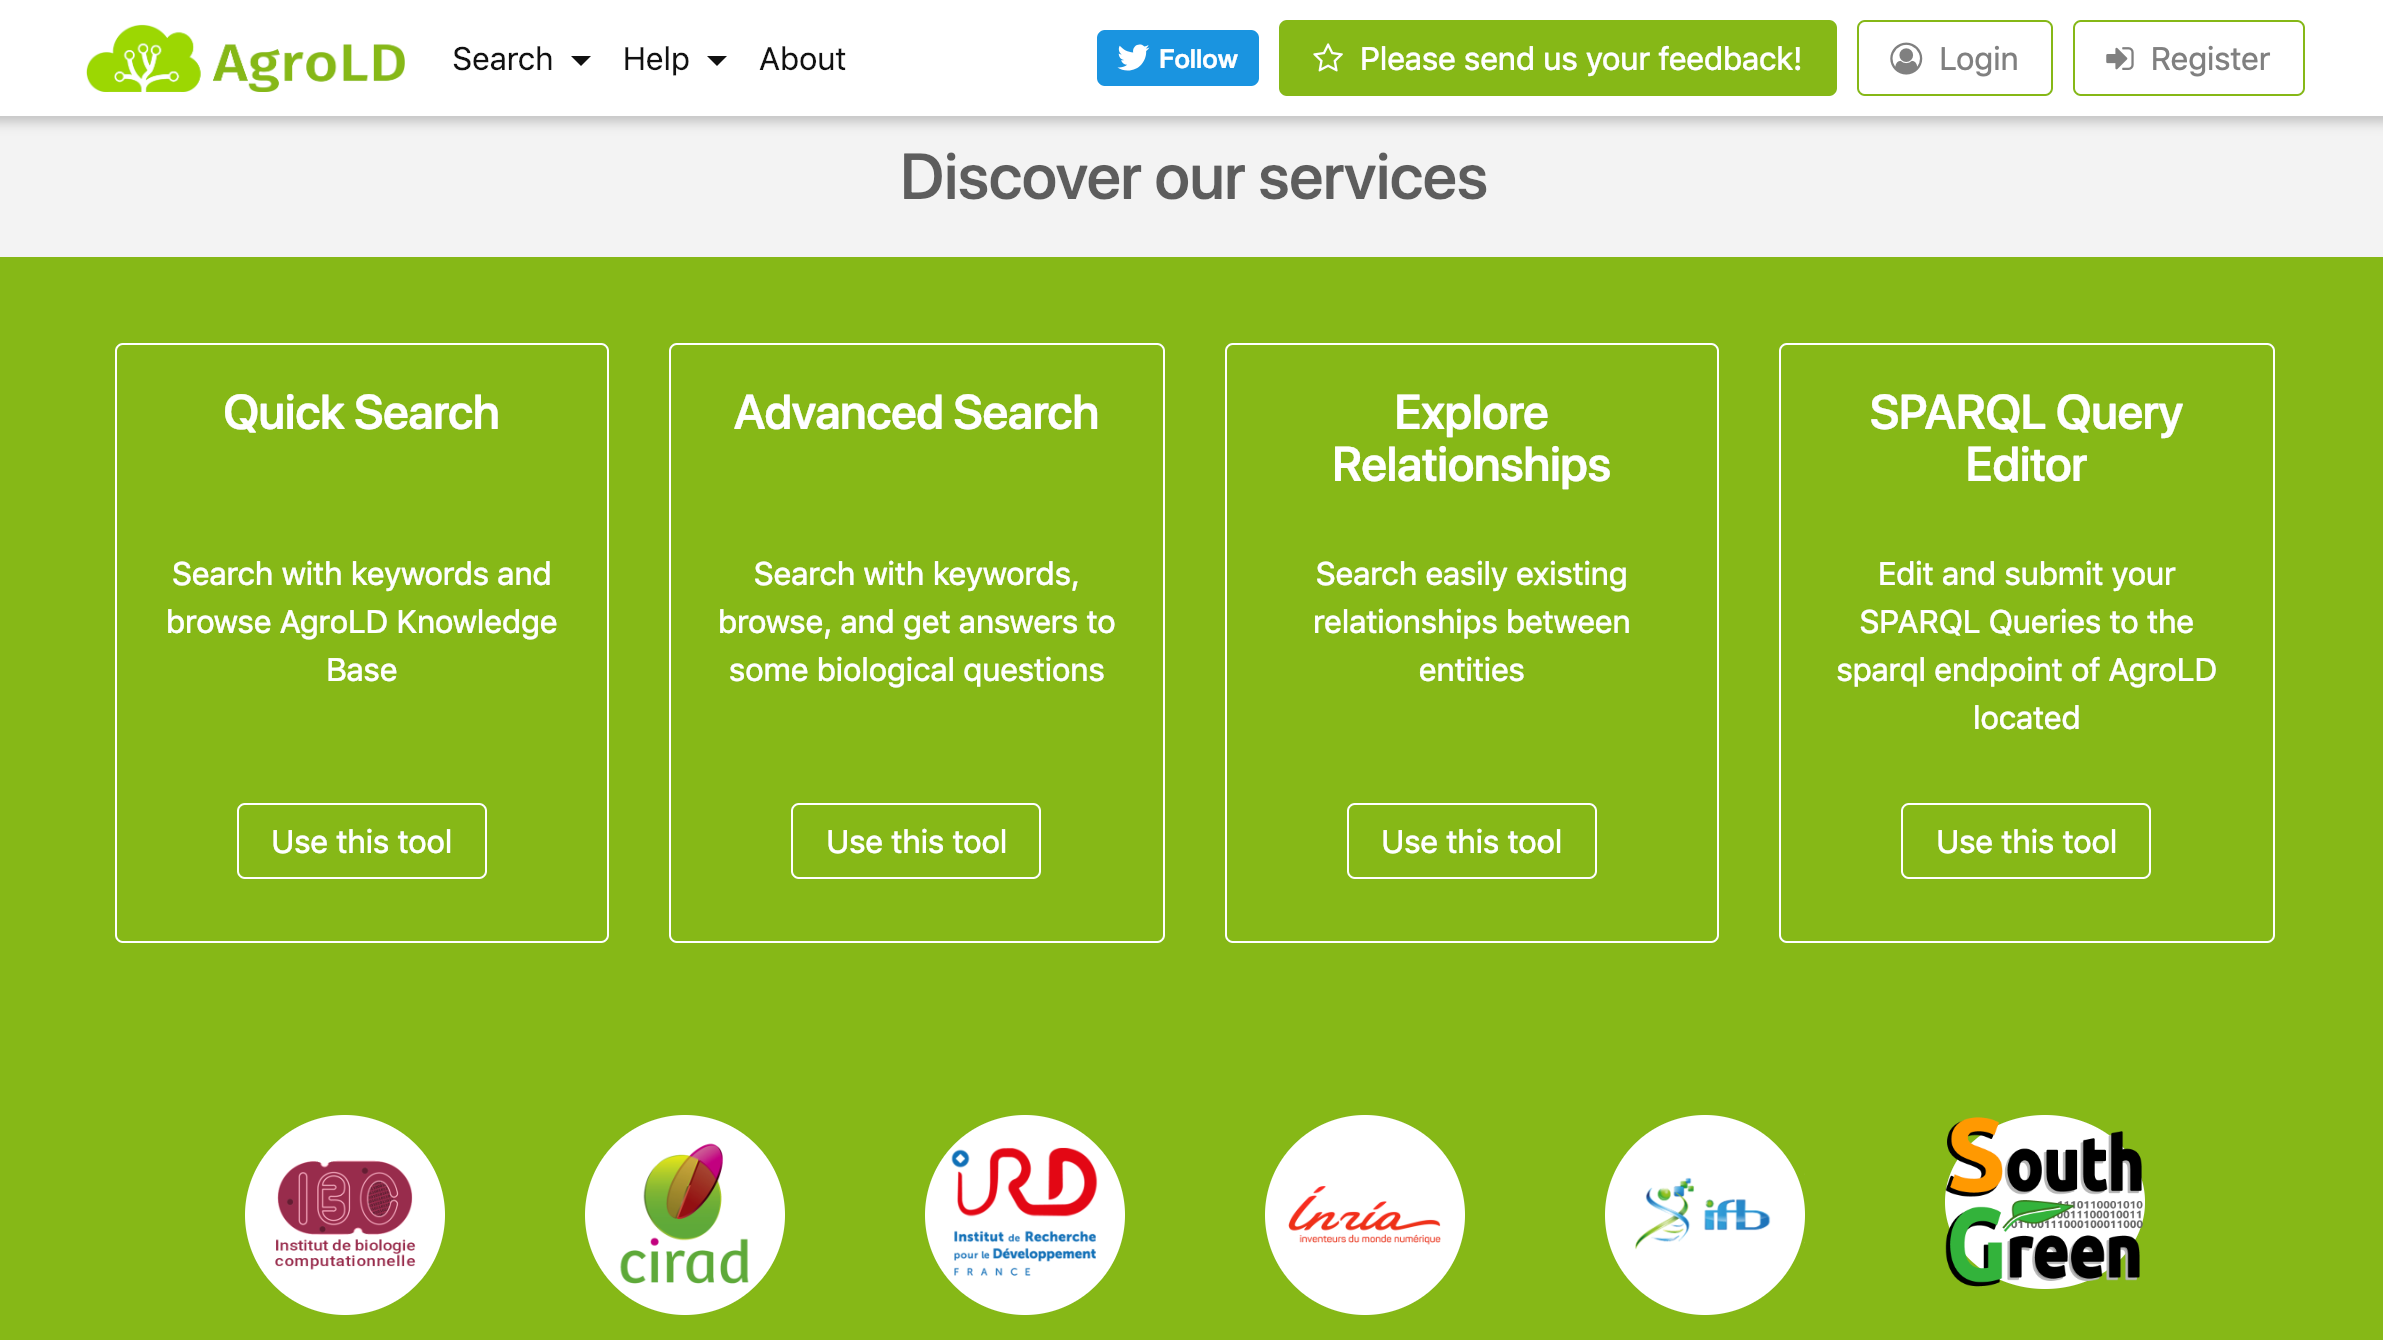
\includegraphics[width=\textwidth]{webapp.png}
\end{frame}


%\begin{frame}{Qui?}
%\end{frame}

\section{Mes missions principales}

\begin{frame}{Maintenance de l'application Web}

\begin{itemize}
	\item Dé-référencement d'URI (adresses web)
	\item Corrections de bugs
	\item Ajout de nouveaux services Web
	\item Mis à jour des librairies utilisées
	\item Gestion de projet: qualité du code, organisation GitHub, passage à Python, ...
	\item etc.
\end{itemize}
\end{frame}

\begin{frame}{Exploration graphique de la base de connaissances}
  \centering 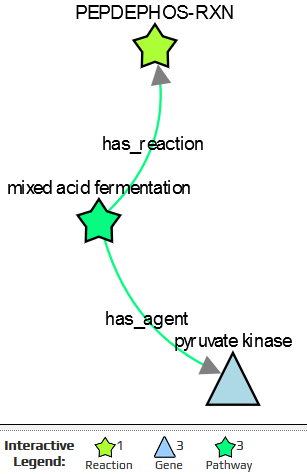
\includegraphics[height=0.7\textheight]{explore-agrold1.png} $\Rightarrow$ 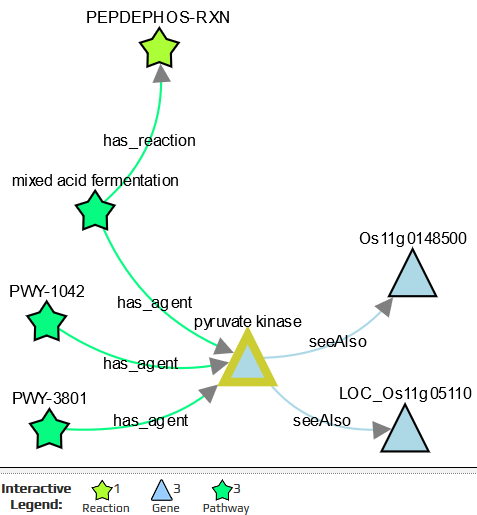
\includegraphics[height=0.8\textheight]{explore-agrold2.png} 
\end{frame}


\begin{frame}{Faciliter l'ajout de services Web} 
\centering 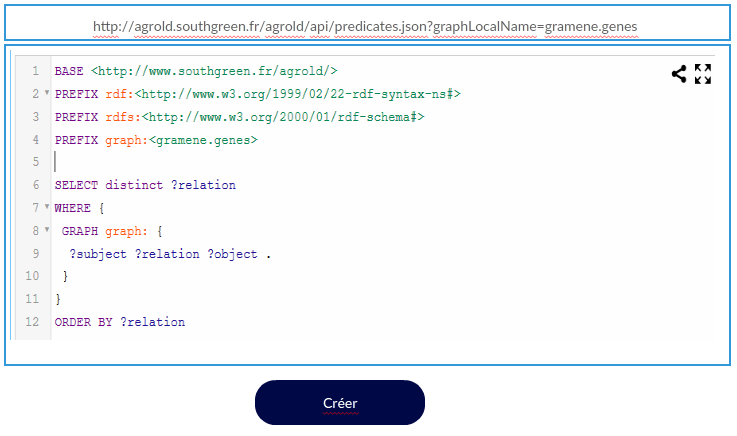
\includegraphics[height=0.7\textheight]{create-webservice.png}
\end{frame}

\begin{frame}{Références sur AgroLD}
\begin{itemize} \scriptsize
	\item Documentation: \url{http://agrold.southgreen.fr/agrold/documentation.jsp}
	\item Code source:   \url{https://github.com/SouthGreenPlatform/AgroLD_webapp}
	\item Code source:  \url{https://github.com/SouthGreenPlatform/AgroLD_ETL}
	\item Aravind Venkatesan, Nordine El Hassouni, Florian Phillipe, Cyril Pommier, Hadi Quesneville, Manuel Ruiz, Pierre Larmande. \textbf{Towards efficient data integration and knowledge management in the Agronomic domain. APIA}: Applications Pratiques de l'Intelligence Artificielle , Jul \textbf{2015}, Rennes, France. \url{http://pfia2015.inria.fr/actes/index.php?procpage=apia. hal-01176903}
	\item Venkatesan, Aravind, Nordine El Hassouni, Florian Phillipe, Cyril Pommier, Hadi Quesneville, Manuel Ruiz, and Pierre Larmande. \textbf{"Exposing French agronomic resources as linked open data." In IN-OLIVE. 2016}. \url{http://ceur-ws.org/Vol-1546/poster_55.pdf}
	\item Venkatesan, Aravind, Gildas Tagny Ngompe, Nordine El Hassouni, Imene Chentli, Valentin Guignon, Clement Jonquet, Manuel Ruiz, and Pierre Larmande. \textbf{"Agronomic Linked Data (AgroLD): A knowledge-based system to enable integrative biology in agronomy." PloS one 13, no. 11 (2018)}: e0198270. \url{https://doi.org/10.1371/journal.pone.0198270}	
\end{itemize}


\end{frame}

\end{document}
